\documentclass{article}
\usepackage[margin=0.5in]{geometry}\usepackage{tikz}
\begin{document}
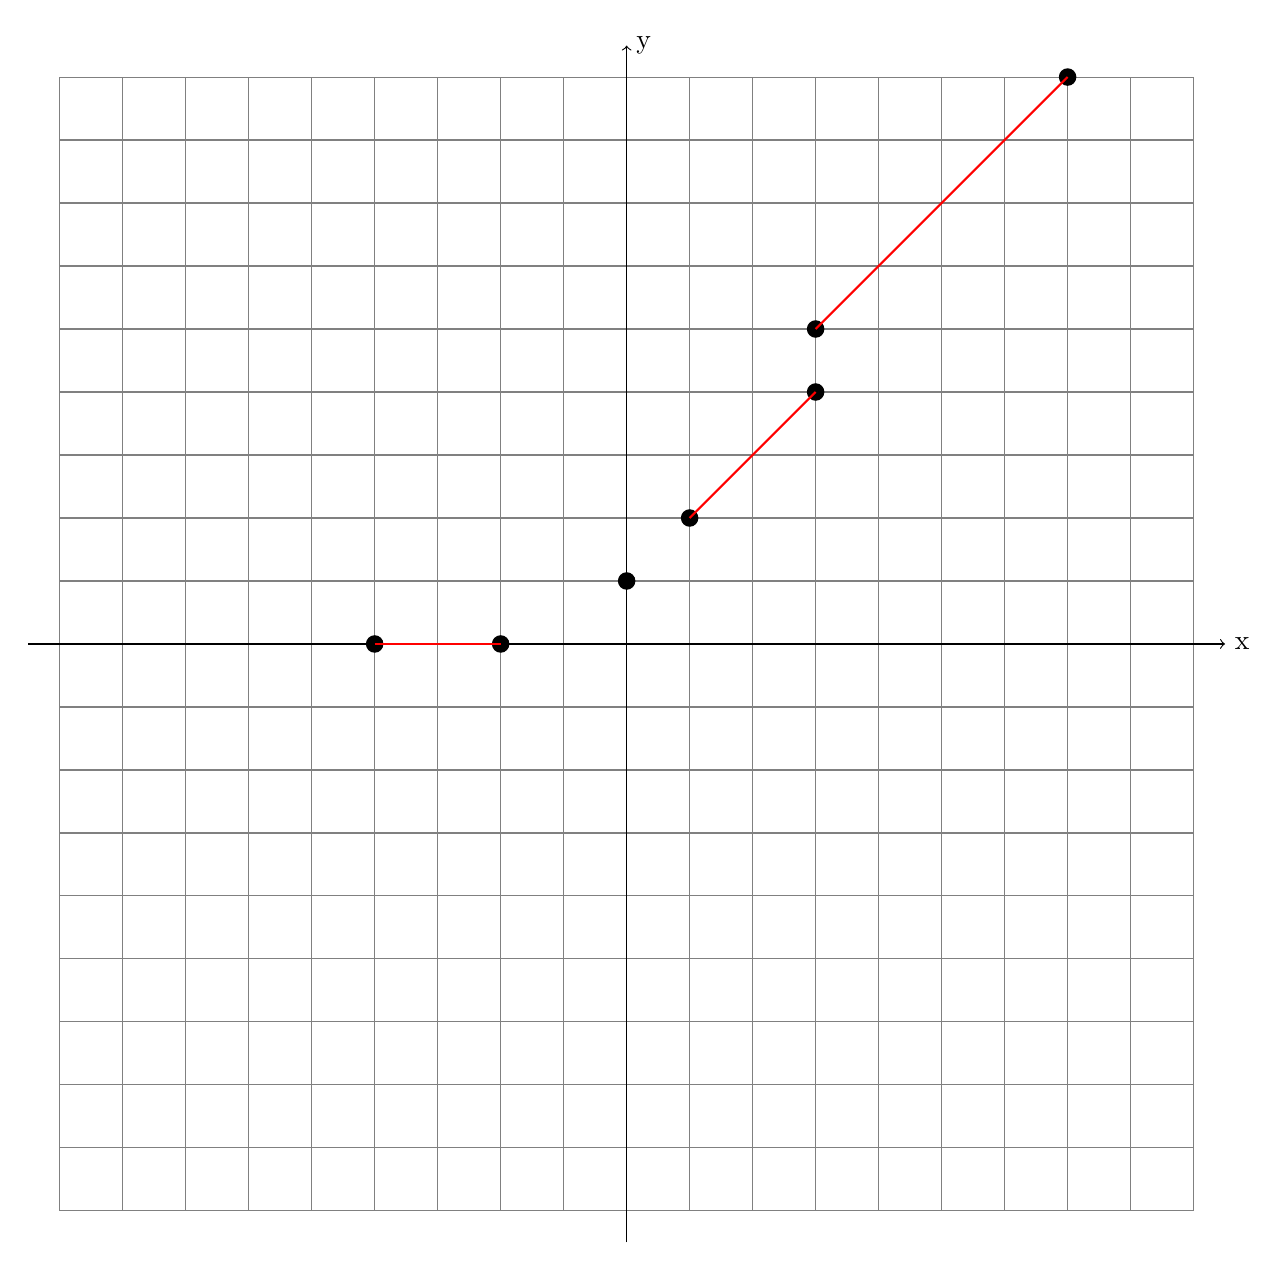
\begin{tikzpicture}[scale=0.800000] % <- Scale picture
   % Coordinate system grid
   \draw[step=1.0,gray,thin] (-9,-9) grid (9,9);
   % Coordinate system axis
   \draw[->] (-9.5,0) -- (9.5,0) node[right] {x};
   \draw[->] (0,-9.5) -- (0,9.5) node[right] {y};
   \draw [fill] (0,1) circle [radius=0.13];
   \draw [fill] (7,9) circle [radius=0.13];
   \draw [fill] (3,5) circle [radius=0.13];
   \draw [thick, red] (7,9) -- (3,5);
   \draw [fill] (-4,0) circle [radius=0.13];
   \draw [fill] (-2,0) circle [radius=0.13];
   \draw [thick, red] (-4,0) -- (-2,0);
   \draw [fill] (1,2) circle [radius=0.13];
   \draw [fill] (3,4) circle [radius=0.13];
   \draw [thick, red] (1,2) -- (3,4);
\end{tikzpicture}
\end{document}
